\documentclass[report.tex]{subfiles}
\begin{document}
\subsection{Theoretical background}

Impedance matching can be achieved through analytical methods, but graphical methods prove to be most efficient; especially  with the help of Smith charts.

A network with a complex input impedance of $Z_{in}=(455-j227)\Omega$ in a system with the characteristic impedance $Z_0=50 \Omega$ has the have a matching input network. To determine this matching network, the source load ($Z_0$) and the complex conjugate of the input impedance ($Z_{in}^*$) is normalized with respect to $Z_0$.
\begin{equation*}
%\label{eqn:z_in}
z_0=Z_0/Z_0 = 1\Omega
\end{equation*}
\begin{equation*}
z_{in}^*=Z_{in}^*/Z_0=(9.1-4.54)\Omega
\end{equation*}
Then, by following the resistance and conductance lines of the Smith chart \emph{from} the normalized source load \emph{to} $z_{in}^*$, as shown in fig.~\ref{fig:input_matching_smith_chart}, the reactance of the matching network is determined by point A. In this case $X_C=$

\begin{figure}[h]
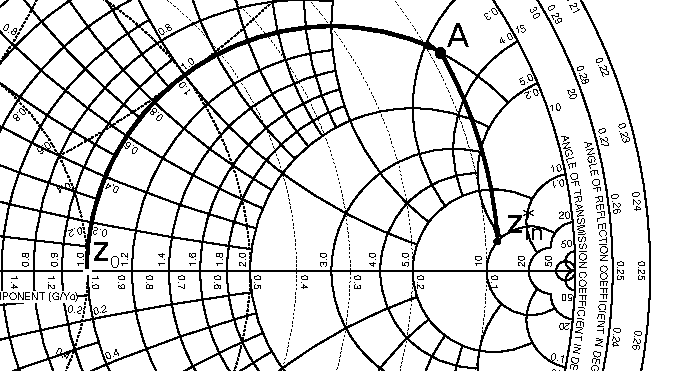
\includegraphics{input_matching_ZY_chart_ver2}
\caption{Input matching in Smith chart}
\label{fig:input_matching_smith_chart}
\end{figure}

\end{document}
